\apendice{Especificación de diseño}

\section{Introducción}
En esta sección se explican todos los aspectos relevantes sobre el diseño de la herramienta como el diseño de la arquitectura o los tipos de datos que se utilizan.

\section{Diseño de datos}
Los datos que se utilizan en la herramienta son los siguientes:
\begin{itemize}
	\item Archivos.py: Se utilizan los códigos hechos en lenguaje python de estos archivos para hacer su análisis.
	\item Archivos.csv: Se forma una matriz dentro de estos archivos para hacer la ponderación de operaciones. 
	\item ByteCode: Es el código intermedio que surge tras compilar el codigo de alto  nivel de los archivos.py.
	
\end{itemize}


\section{Diseño procedimental}
A continuación se verán las interacciones entre los elementos de la herramienta:

\begin{figure}[H]
\centering
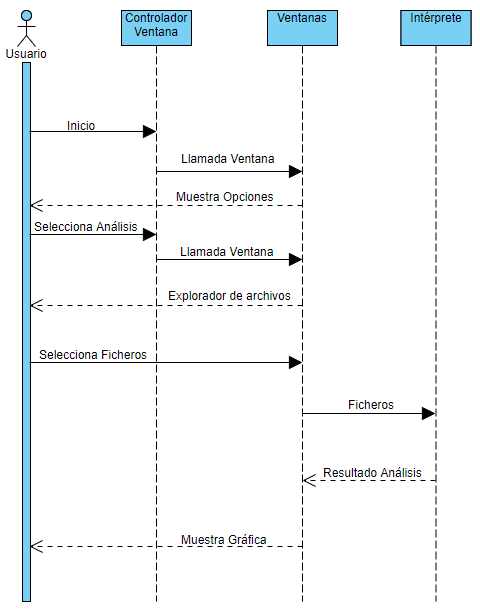
\includegraphics[width=9cm, height=12cm]{Secuencia}
\caption{Diagrama secuencial de la ejecución de la herramienta}
\end{figure}



Como se puede ver en el diagrama, el usuario tiene una interacción constante con la herramienta en toda su ejecución.
\section{Diseño arquitectónico}
El diseño arquitectónico de la herramienta se basa en un sistema de ventanas que se llaman las unas a la otras y mientras  tanto hay un controlador que gestiona que gestiona las llamadas.

\begin{figure}[H]
\centering
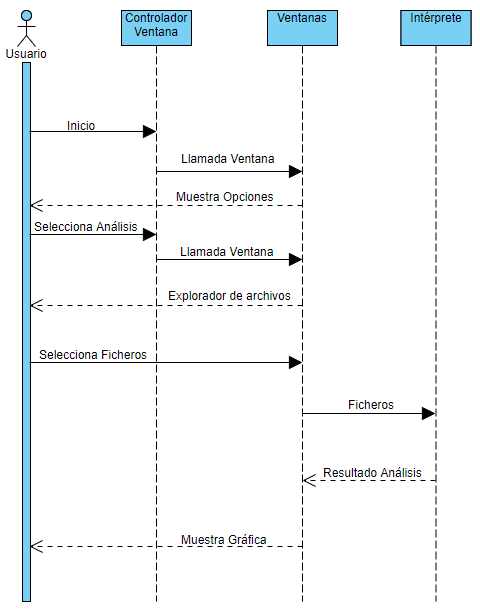
\includegraphics[width=14cm, height=7cm]{Secuencia}
\caption{Diagrama secuencial de la ejecución de la herramienta}
\end{figure}
